%!TEX root = ../../../adrien_gomar_phd.tex

For each row, a single-blade passage meshed
with an O4H topology is used to compute this
CROR configuration as show in Fig.~\ref{fig:dream_mesh}. This is a classical
topology for turbomachinery computations that is here applied to 
a CROR.
\begin{figure}[htp]
  \centering
  \subfigure[Topology]{
    \label{fig:dream_mesh}
    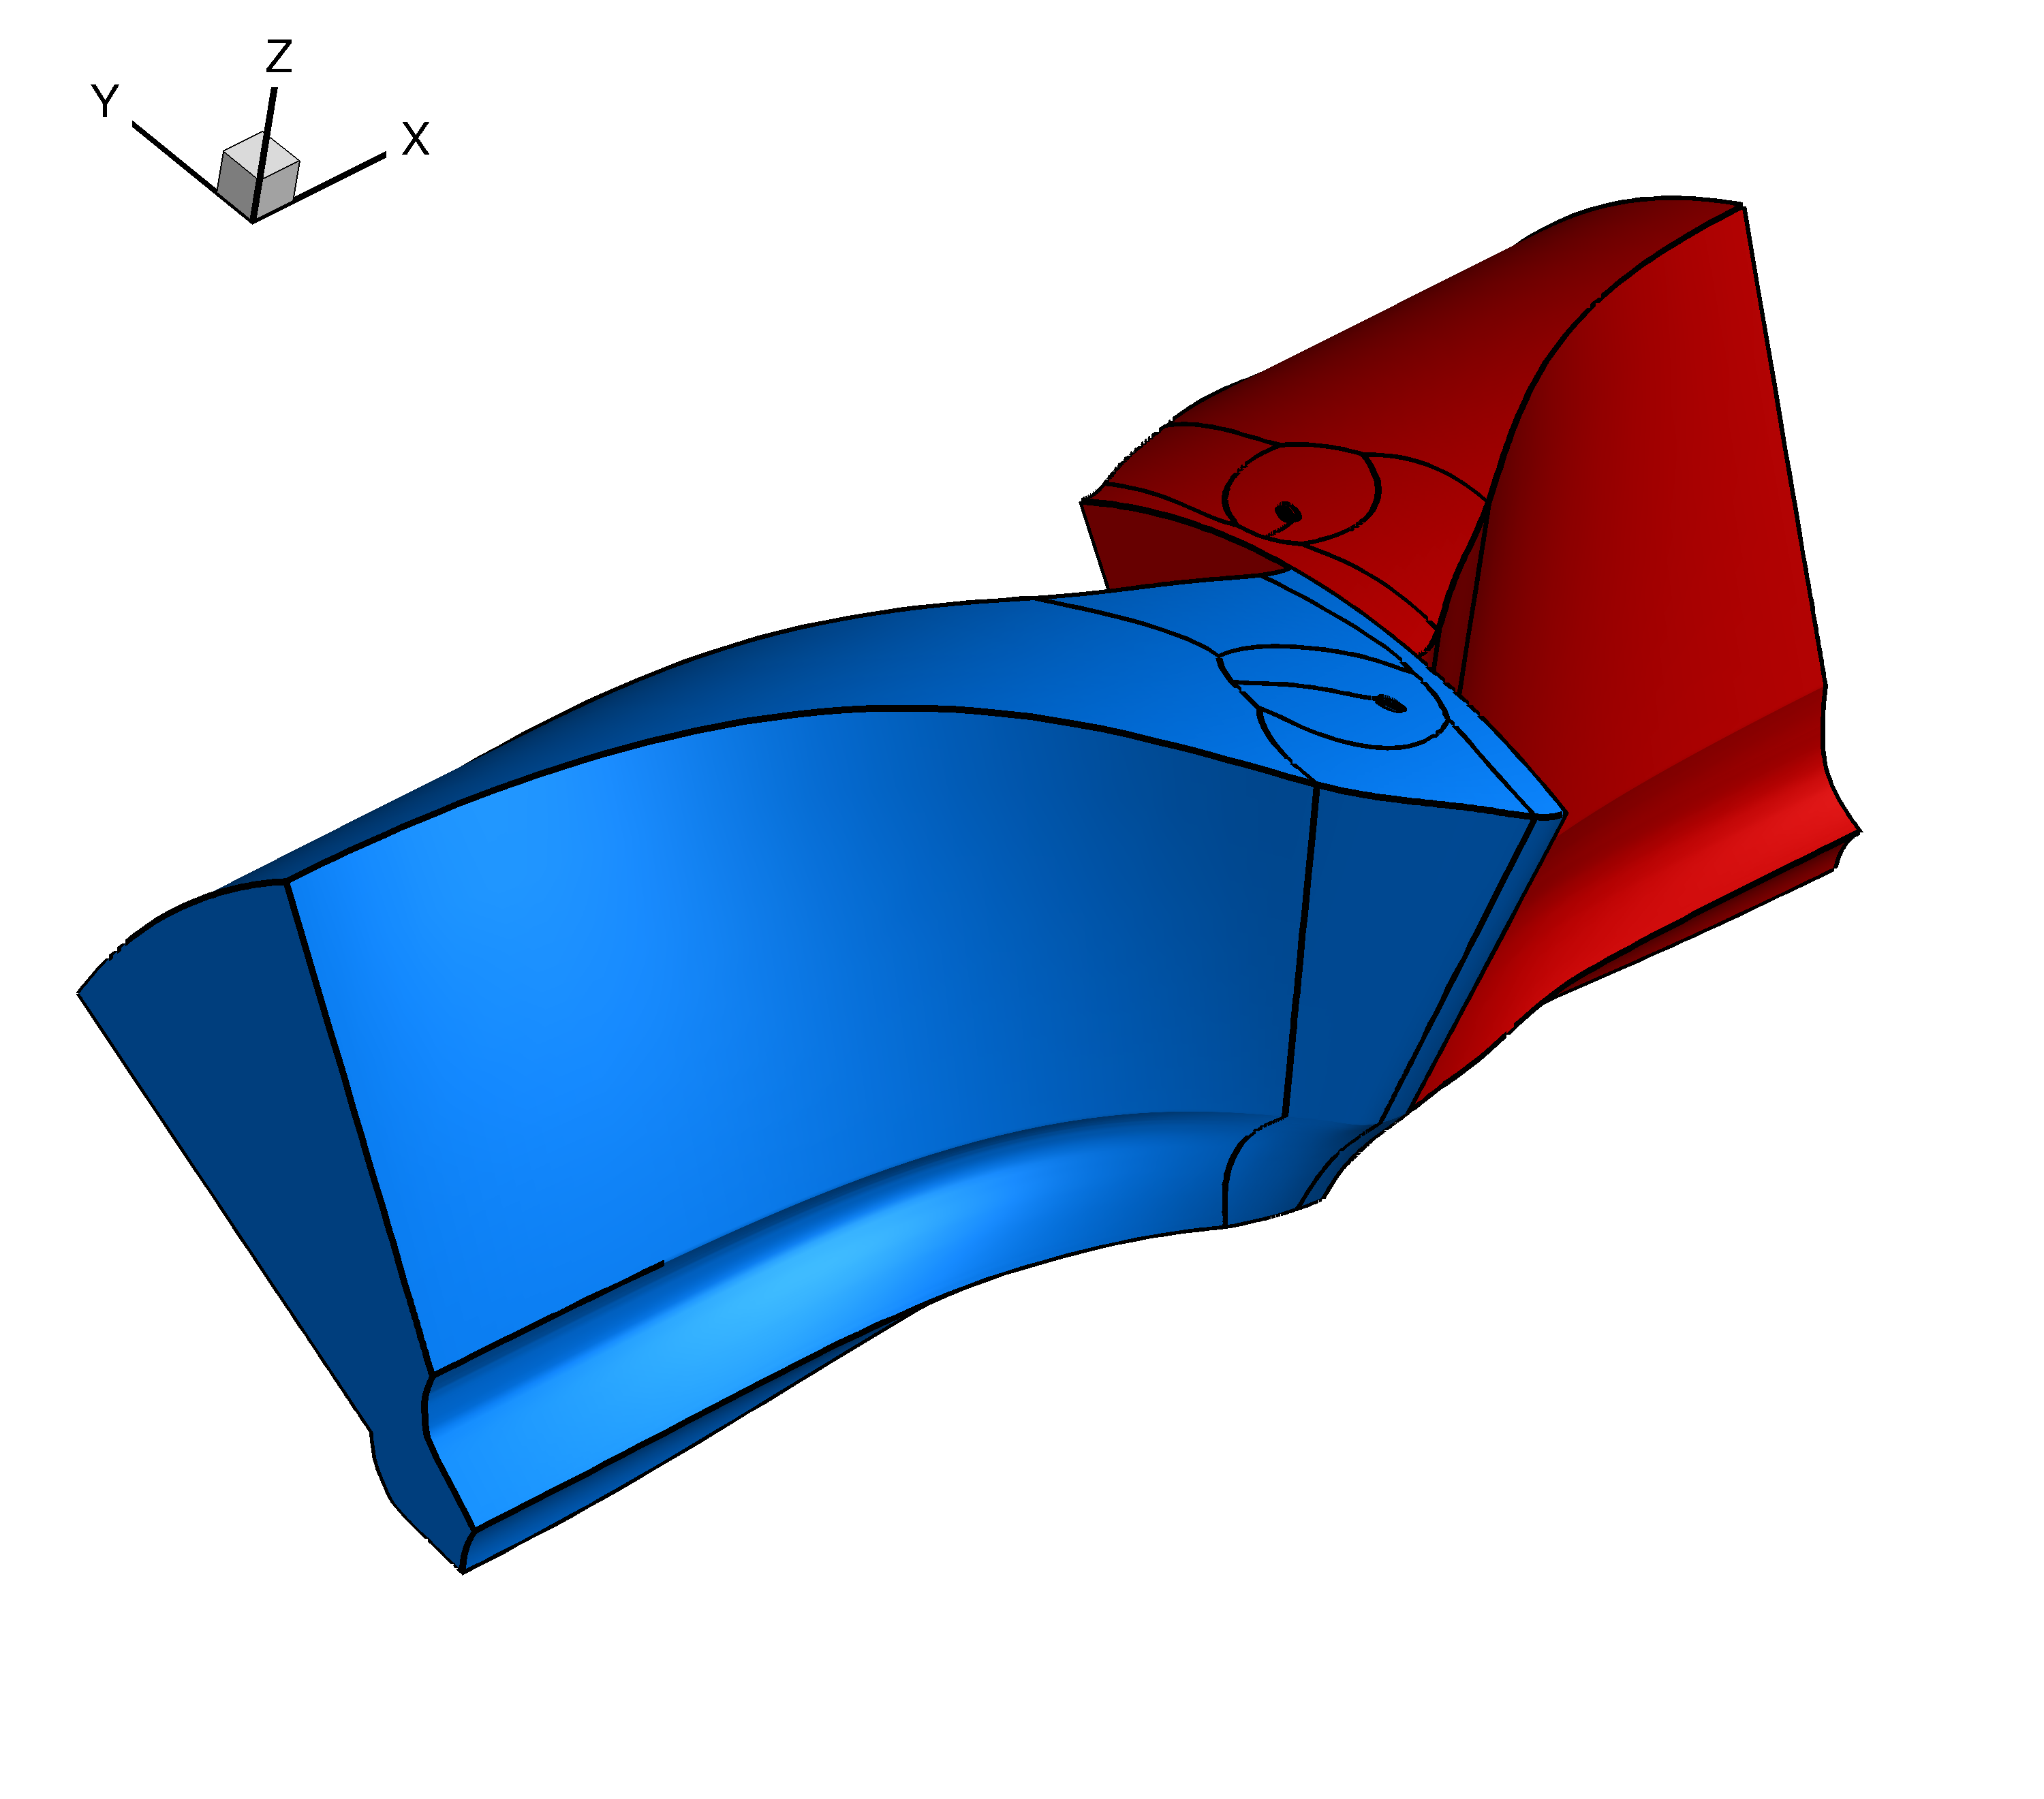
\includegraphics[height=.4\textwidth]{dream_mesh.png}}
  \subfigure[Detailed topology with number of grid points]{
    \label{fig:dream_ls_mesh}
    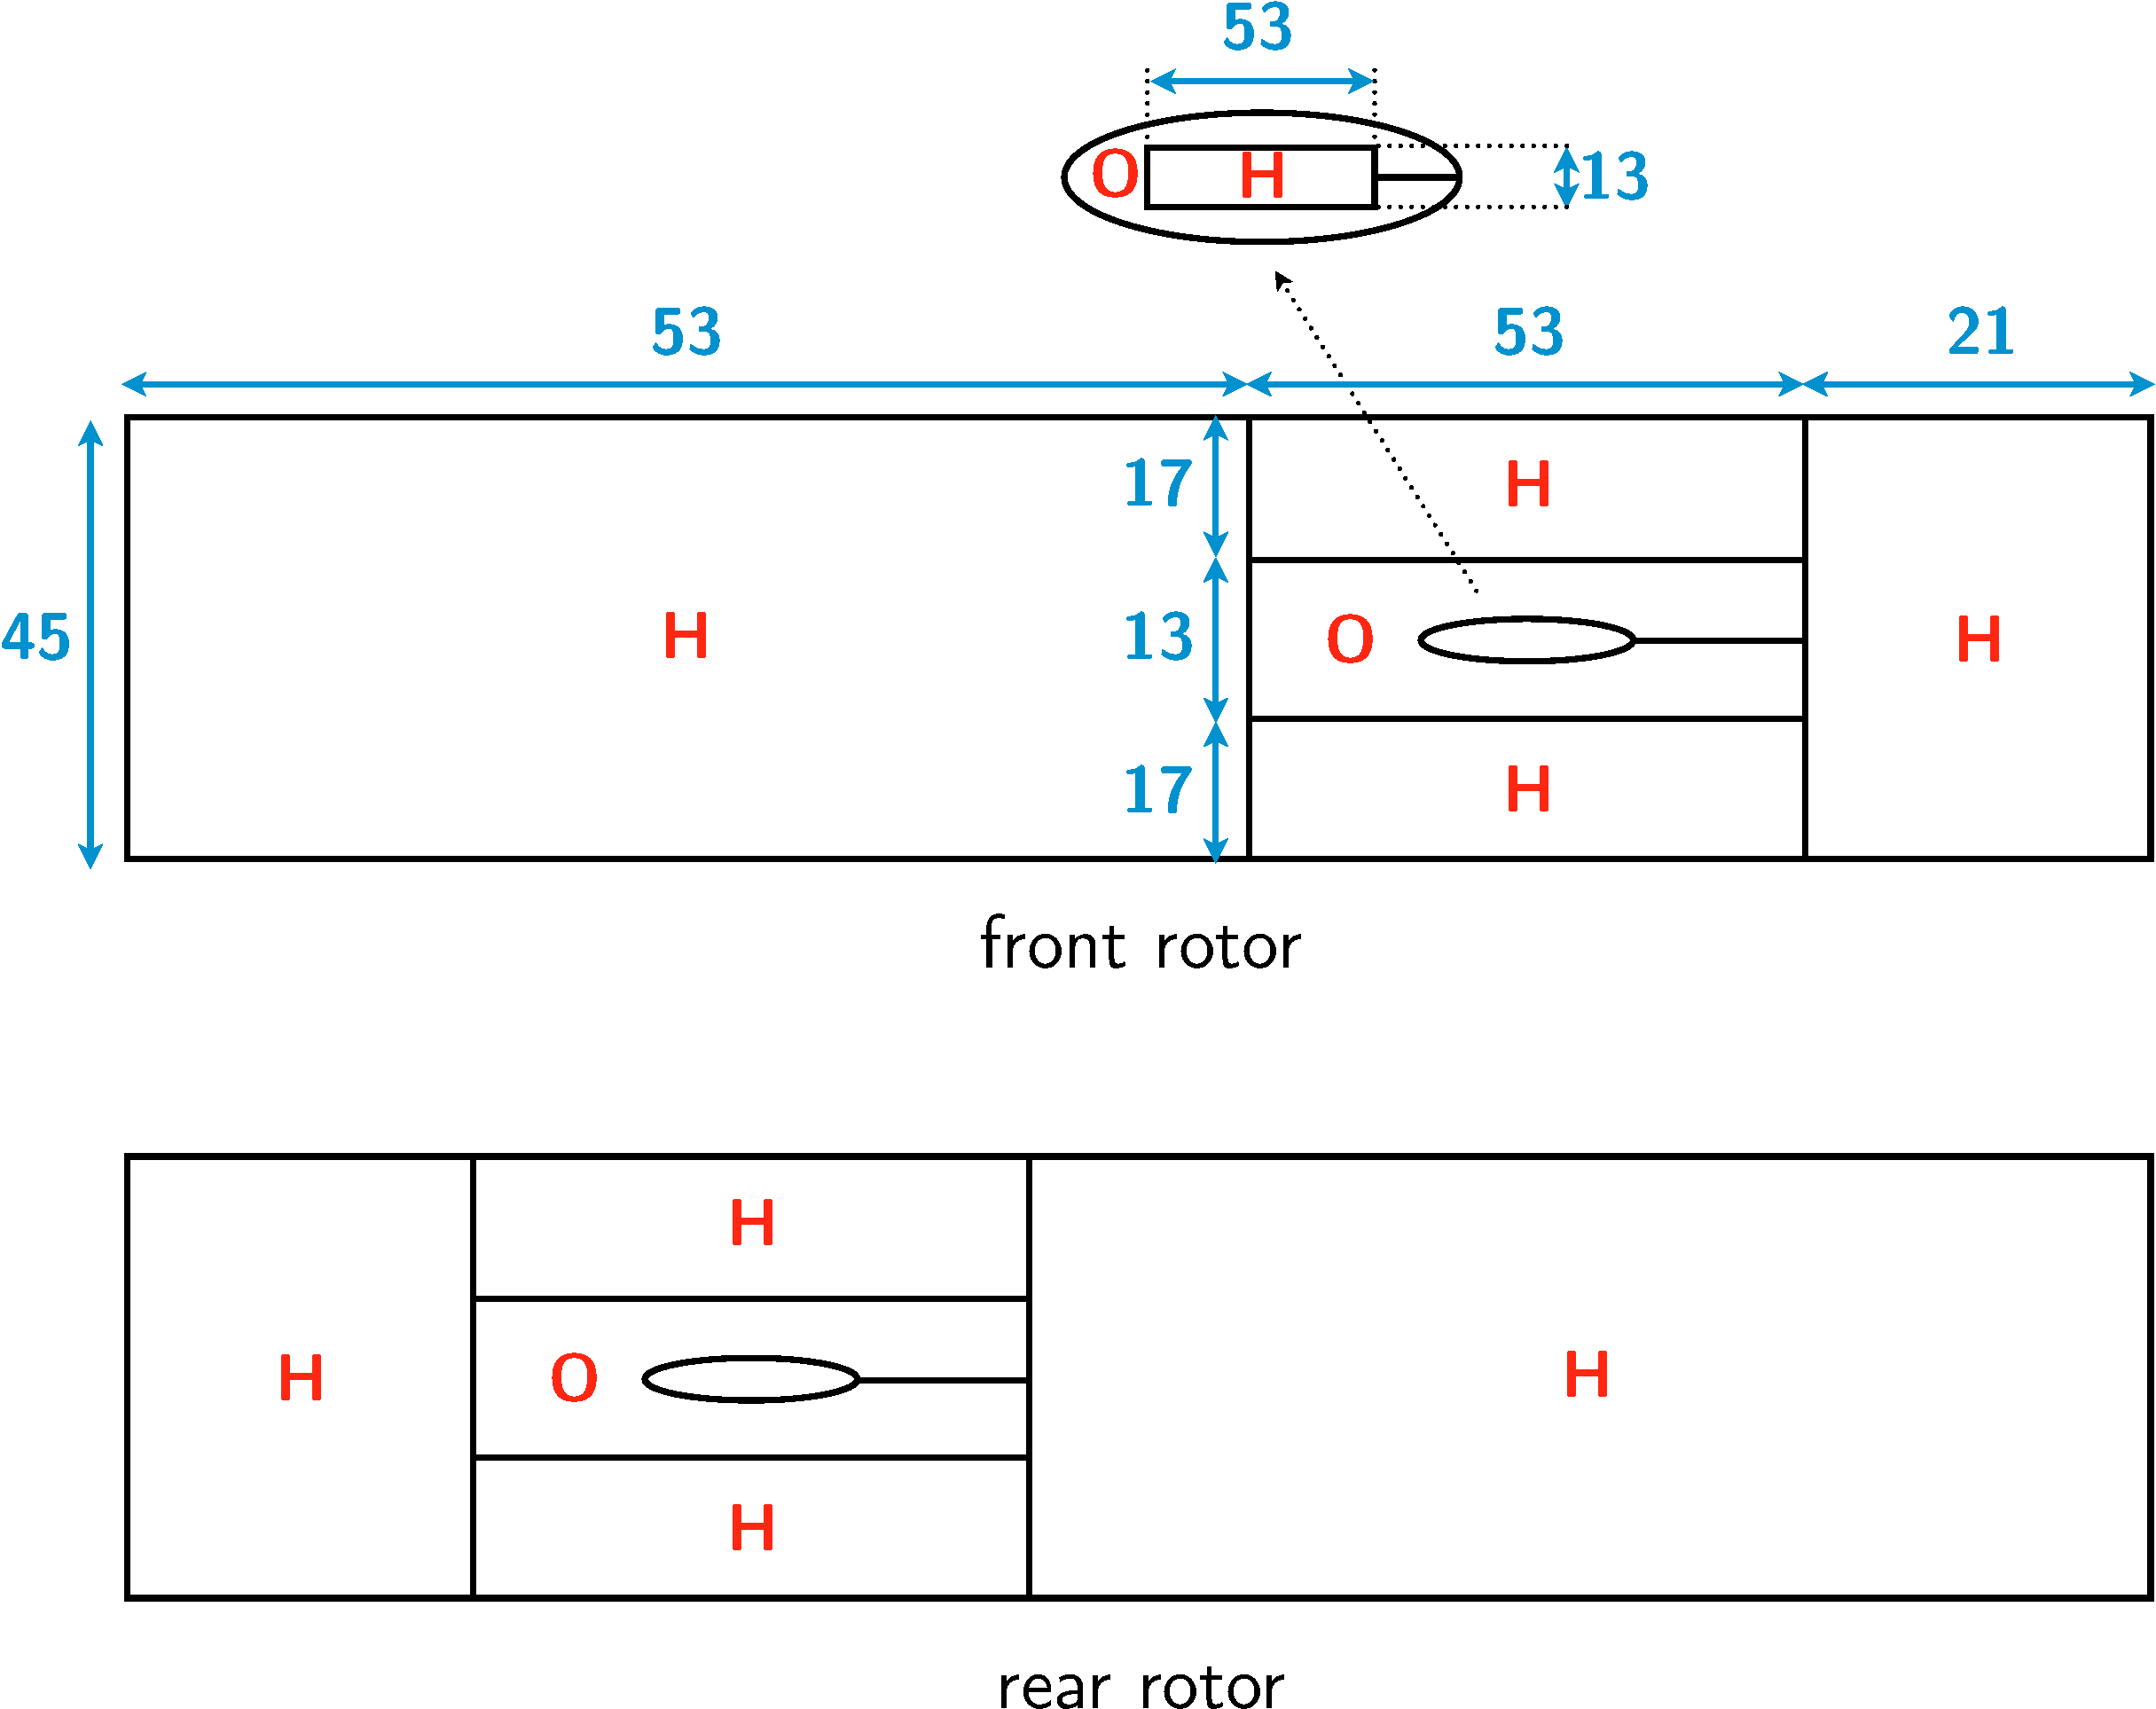
\includegraphics[height=.4\textwidth]{dream_ls_mesh.pdf}}
  \caption{Low-speed isolated configuration mesh topology.}
\end{figure}
The number of points is reported in 
Fig.~\ref{fig:dream_ls_mesh} for a blade-to-blade section. 
129~points discretize the blade, 45~the pitch and 181~the radial
extent. The same number of grid points is used for the front
and the rear rotor blades. 
Finally, the total number of grid points is almost $5$ million, which
is consistent with the literature values~\cite{Stuermer2008,Bechet2011,
Francois2013,Zachariadis2011,Peters2012}.

As a CROR is not shrouded, a sufficiently large
far-field domain is taken to ensure a minimum influence
of the far-field boundary conditions on the results.
The computational domain is schematically reproduced 
in Fig.~\ref{fig:dream_farfield}.
The radial extent is $3D$ while the axial one is $3.5D$, with
$D$ being the diameter of the front rotor.
In the literature, 
\citet{Peters2012} consider an axial extent of $7.5D$
with a radial extent of $4D$ while \citet{Zachariadis2011}
consider $2.5D$ and $3.6D$, respectively. We are thus in 
the mid-range of the values taken in the literature.
\begin{figure}[htp]
  \centering
  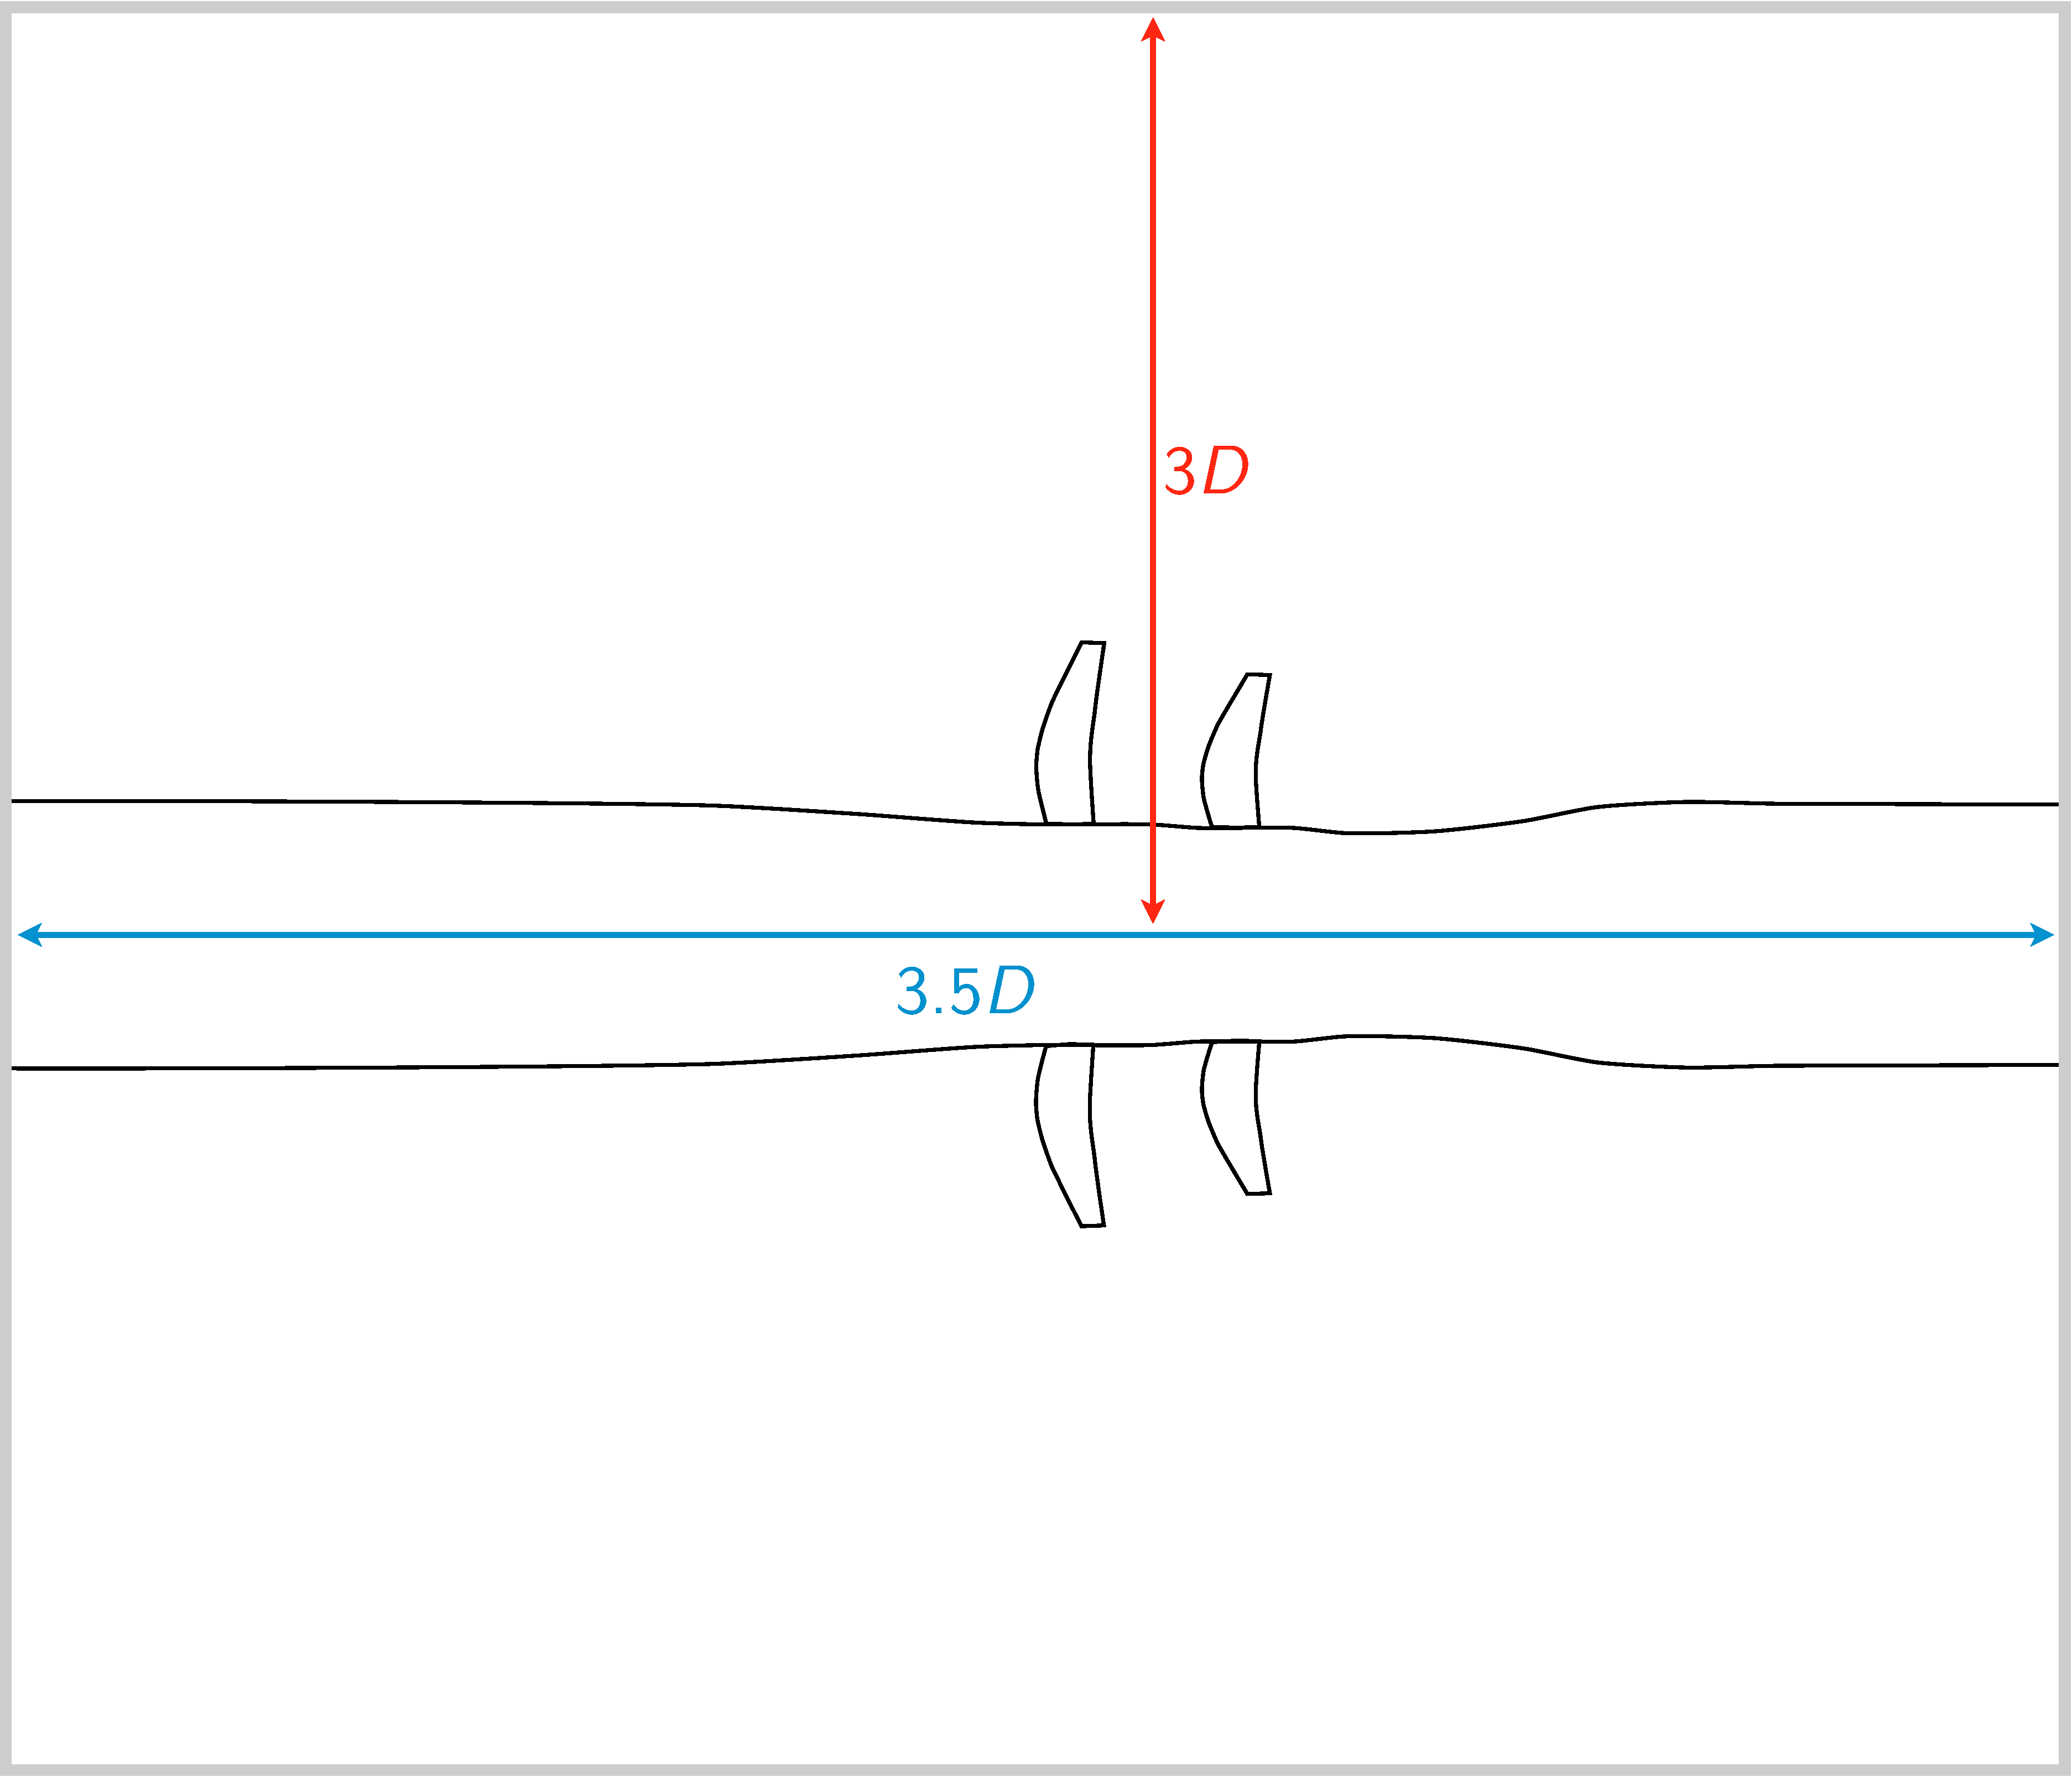
\includegraphics[width=.4\textwidth]{dream_farfield.pdf}
  \caption{Low-speed isolated configuration far-field domain and boundary conditions.}
  \label{fig:dream_farfield}
\end{figure}
As highlighted by the underlined text in Fig.~\ref{fig:dream_farfield},
the boundary conditions used here are: (i)~adiabatic walls
for the blades and the shroud (or spinner), (ii)~constant
stagnation values used at the far-field, (iii)~periodic
or phase-lagged for the azimuthal boundaries of the channel
and (iv)~a mixing-plane or a sliding mesh interface is
used depending on the type of computation (steady or unsteady).
In opposite to the mesh convergence study made previously on the STCF11
configuration (see Sec.~\ref{sec:stcf11_numerical}),
the mesh stems from literature and industrial best
practices and will thus not be assessed.

Turbulence is modeled using the one-equation model of
\citet{Spalart1992}.  Roe's scheme~\cite{Roe1981} along with a 
second-order MUSCL extrapolation 
is used to compute the convective fluxes.
The maximum CFL number is set to~10 for the steady 
computations and to~5 for the unsteady simulations.

\paragraph{Influence of the spatial discretization}
\label{sub:dream_ls_spatial_discretization}

To assess the influence of spatial discretization, four 
space schemes are used to simulate the low-speed CROR configuration.
These four schemes are the \citet{Jameson1981} scheme (noted JST) with artificial
viscosities $\kappa_4 = 0.016$, $\kappa_4 = 0.032$, $\kappa_4 = 0.064$
and $\kappa_2$ equal to $0.5$ as the operating point (low-speed
flight condition) should not 
lead to shocks. In addition to this scheme, three upwind
Roe's schemes~\cite{Roe1981} along with no extrapolation (noted Roe~1),
a second order (noted Roe~2) or a third-order (noted Roe~3) 
MUSCL extrapolation are used.

The convergence of the different computations is show 
in Fig.~\ref{fig:dream_ls_space_scheme_residual}
for the four schemes. The convergence is not 
very good. Only the Roe~1 and Roe~2 spatial schemes give 
a convergence that has an acceptable slope. In contrary,
the JST~$\kappa_4 = 0.016$ diverges and the three
remaining schemes hardly converge. The higher the
viscosity parameter $\kappa_4$ of the JST scheme, the better
the convergence. Exceeding $\kappa_4 = 0.064$ should
warn us that something might be wrong with the computation.
As stated previously, this is actually due to the range of Mach
number in which this low-speed configuration operates. In fact,
a part of the computation can be said to be within the incompressible
range ($M \leq 0.3$) and therefore not adapted to a compressible
flow solver which is the case of the \emph{elsA} code 
(see Appendix~\ref{app:elsa}).
\begin{figure}[htp]
  \centering
  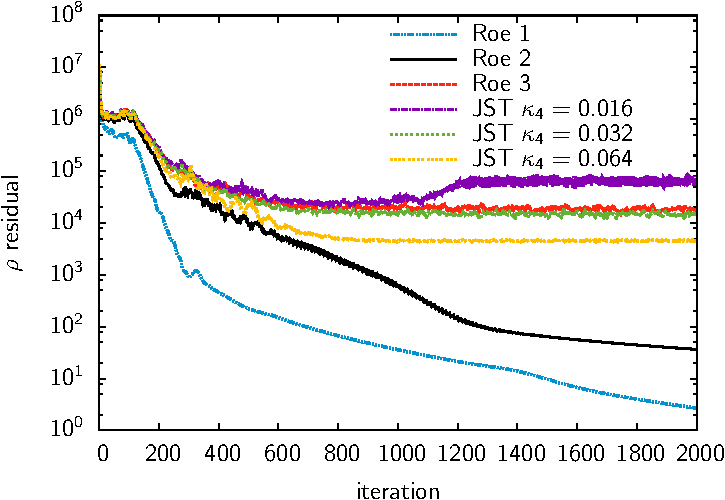
\includegraphics[width=.5\textwidth]{SPACE_SCHEME_DIFF_LS_RESIDUALS.pdf}
  \caption{Low-speed isolated configuration: convergence of the
  steady computations using different spatial schemes.}
  \label{fig:dream_ls_space_scheme_residual}
\end{figure}

To further differentiate the spatial schemes, 
the steady results for the similarity coefficients are reported
in Fig.~\ref{fig:dream_ls_space_scheme_coeff} for all spatial scheme, 
except the diverging JST~$\kappa_4 = 0.016$ computation.
The results are normalized by the Roe~2 values.
The Roe~2, Roe~3, and the two JST schemes give equivalent
similarity coefficients as the difference is smaller than 1~\%.
In opposite, the first order upwind scheme Roe~1 give a 5~\%
difference for both the traction coefficient $C_T$ and the efficiency $\eta$.
Cross-comparing these results with the convergence of the computations
reported in Fig.~\ref{fig:dream_ls_space_scheme_residual}, the Roe~2
scheme is kept for the following as it give both a good convergence
of the residuals and consistent similarity coefficients.
\begin{figure}[htp]
  \centering
  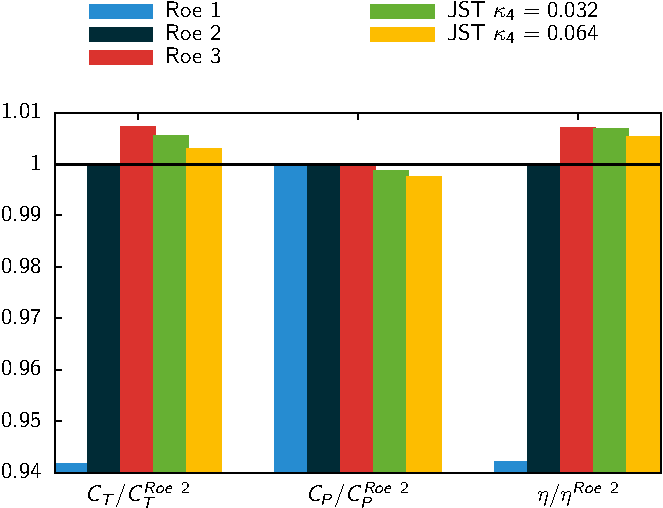
\includegraphics[width=.5\textwidth]{SPACE_SCHEME_DIFF_LS_COEFF.pdf}
  \caption{Low-speed isolated configuration: convergence of the 
  similarity coefficients using different spatial schemes.}
  \label{fig:dream_ls_space_scheme_coeff}
\end{figure}

\paragraph{Aeroelastic simulations}
\label{sub:dream_ls_ael_presentation}

Two structural modes are considered for the aeroelastic study of this 
configuration: the second bending/flexion mode and the first torsion mode
of the front rotor. These were inputs of the current work.
The shape of the modes is shown in Fig.~\ref{fig:dream_ls_ael_modes}
with an arbitrary amplitude, large enough to ease the visualization.
Two inflection lines are seen for the 2F mode, while only
one is seen for the 1T, hence their designation.
\begin{figure}[htp]
  \centering
  \subfigure[2F]{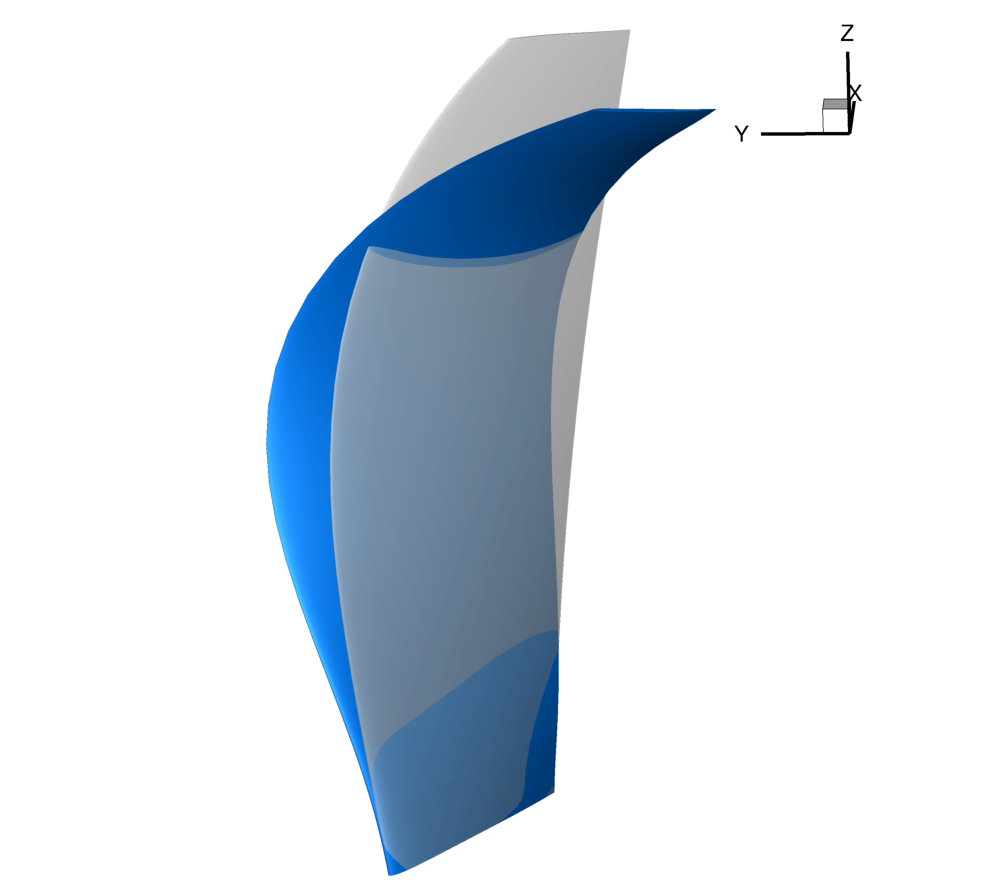
\includegraphics[height=.35\textwidth]{mode_2F.png}}
  \subfigure[1T]{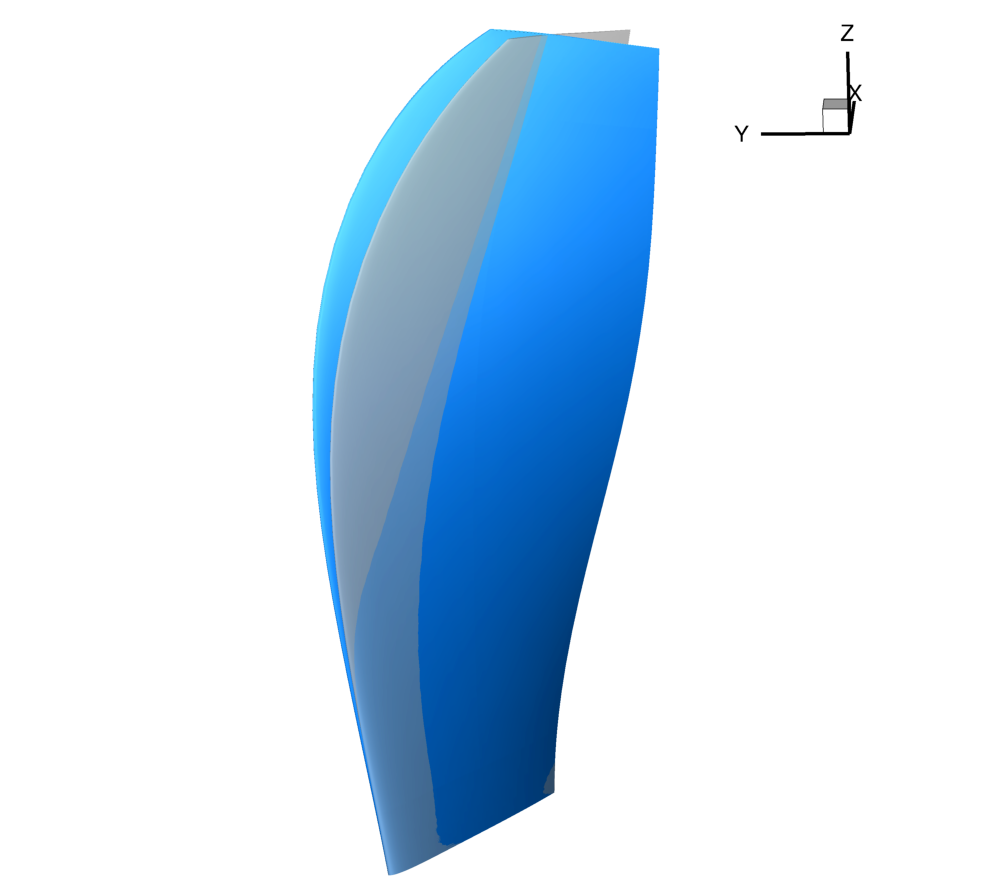
\includegraphics[height=.35\textwidth]{mode_1T.png}}
  \caption{Low-speed isolated configuration: structural modes considered.}
  \label{fig:dream_ls_ael_modes}
\end{figure}
The frequency, mass and stiffness of the modes 
are given with the corresponding modes.
The frequency of each modes varies between 
$495~\textrm{Hz} \leq f_{AEL} \leq 600~\textrm{Hz}$
while the blade passing frequency of the opposite rows,
namely the rear rotor, is $1913~\textrm{Hz}$. However,
this last frequency governs the unsteady rigid flow physics 
and will have to be computed along with the aeroleastic frequency.
Therefore, the multi-frequential formulation of the
harmonic balance approach will be used in the following.

The AEL module of the \emph{elsA} CFD flow solver is used.
Again, only a one-blade passage domain is meshed.
Phase-lag boundary conditions are therefore used
and each computed frequency is associated to one phase-lag~\cite{ThesisGuedeney}.
For the aeroelastic modes, 
four nodal diameters are considered, corresponding to IBPA
values of: $[-60^\circ, -30^\circ, 30^\circ, 60^\circ]$. 
The aeroelastic coupling is considered to be linear (weak coupling
approach), therefore a very small amplitude of the mode is applied
and the fluid response is analyzed.

Due to the non-linearity of the Navier--Stokes
equations, combinations of 
the two base frequencies (blade passing frequency and
aeroelastic frequency) can emerge in the front rotor. 
This leads to a set of possible frequencies that 
is two-dimensional. An infinite number of frequencies
can not be computed meaning that this set 
has to be truncated. In the electronic literature,
\citet{Kundert1988} propose two types of truncation:
the "square grid" and the "diamond grid" truncations.
These are schematically represented in Fig.~\ref{fig:dream_hb_truncation}.
Dots represent frequencies that are computed by the multi-frequential
harmonic balance approach.
\begin{figure}[htp]
  \centering
  \subfigure[square grid]{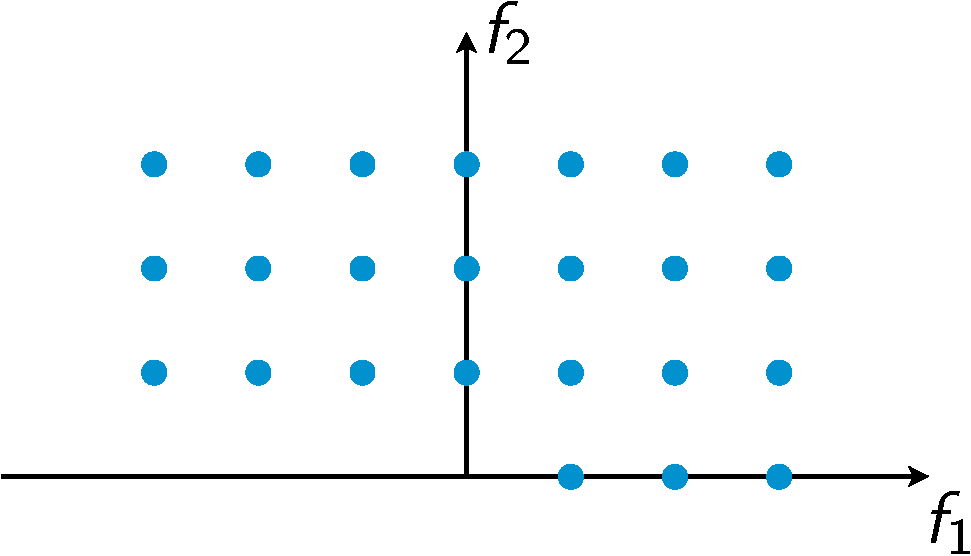
\includegraphics[width=.25\textwidth]{truncation_square.pdf}}
  \subfigure[diamond grid]{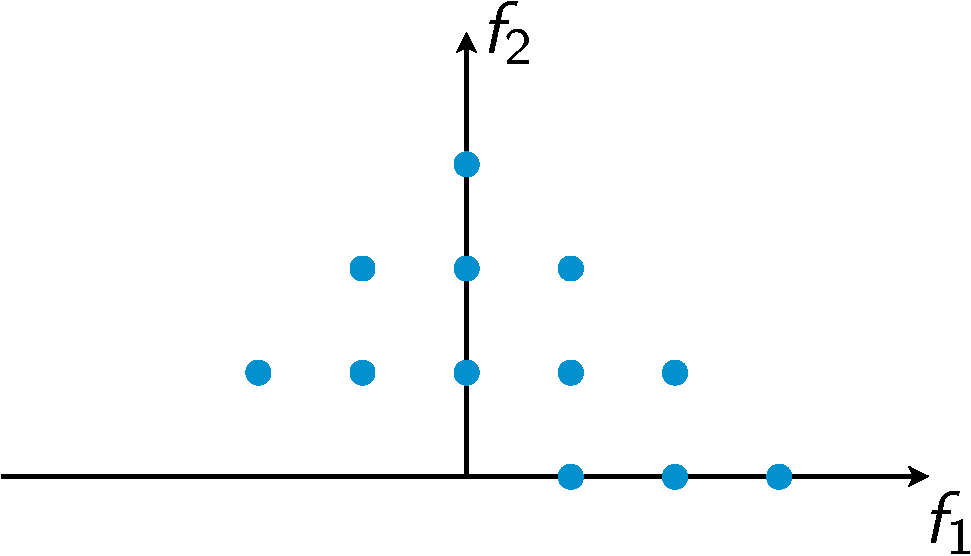
\includegraphics[width=.25\textwidth]{truncation_diamond.pdf}}
  \subfigure[cross grid]{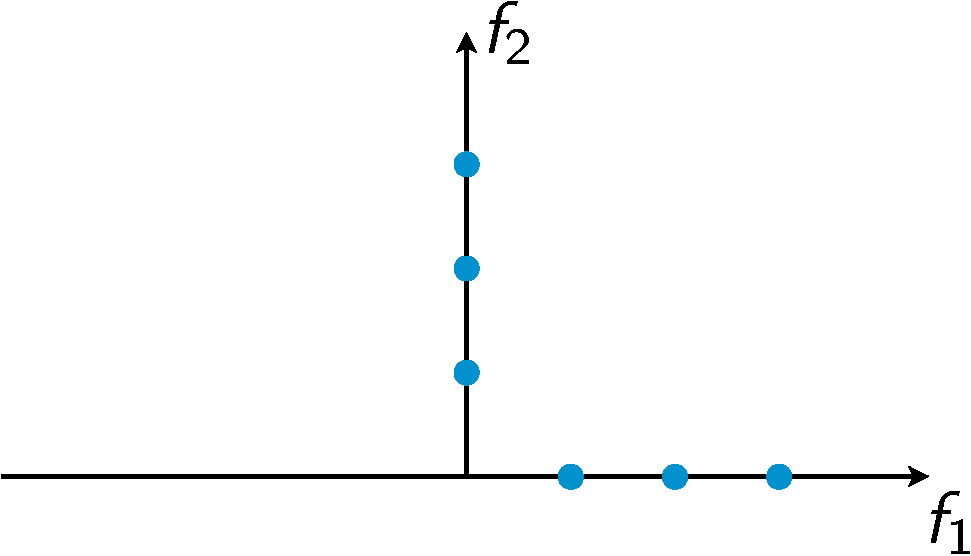
\includegraphics[width=.25\textwidth]{truncation_cross.pdf}}
  \caption{Truncation grids for reducing the set of frequencies of multi-frequential
  harmonic balance computations.}
  \label{fig:dream_hb_truncation}
\end{figure}
In the turbomachinery literature, \citet{Gopinath2007} follows the
diamond grid pattern while \citet{Ekici2007} seems to choose a
square grid pattern. In his PhD thesis, \citet{ThesisGuedeney}
first choose the frequencies by knowing which one emerge based on
a reference classical time-marching computation. Of course,
this approach can only be done \emph{a posteriori} which limits
the predictability of the method. He
also made computations with a "cross grid" truncation 
(shown in Fig.~\ref{fig:dream_hb_truncation}), this new type 
of truncation scheme only considers the harmonics of the
base frequencies. \citet{ThesisGuedeney} showed that this
truncation pattern gives
similar if not better results that the
"diamond grid" truncation pattern. 

In this work, the two frequencies 
have a different physical meaning. In fact, while the blade passing frequency
has been shown to convey the main flow physics (potential effects, wakes, 
tip vortices to name but a few), the aeroelastic frequency is more likely
to influence the near blade wall flow field. In fact, as recalled
previously, the amplitude of vibration is kept very small,
yielding a local influence of the blade vibration.
Therefore, in this work, it seems reasonable to choose a "cross grid"
truncation pattern.

Finally, the harmonic balance computations are run with
five frequencies in total. In the rear rotor,
the harmonics of the front rotor blade passing frequency
are chosen. In the front rotor, the first frequency is the
frequency associated to the vibration of the blade and the
remaining ones are harmonics of the rear rotor blade 
passing frequency.

The time instances are automatically chosen using the OPT
algorithm (see Sec.~\ref{sec:algo_opt}) which leads to 
a condition number always lower than $1.1$ which ensure
the convergence of the computations.